\documentclass[10pt]{article}
\usepackage[margin=0.75in]{geometry}
\usepackage{graphicx}
\usepackage{hyperref}
\usepackage{booktabs}
\setlength{\parindent}{0pt}
\setlength{\parskip}{6pt}
\begin{document}
\section*{n47 polynomial00 blocked D5: terminal record}
The fixed attempt ended with \texttt{projection\_kills\_one} in the degree-five quotient and emitted no D5 certificate. The independent D4 checker accepted $1\notin W_4(F)$ with codimension at least 21,428; a fresh exact counter found zero solutions. This certifies last fall degree at least 5 for the named Boolean presentation under the frozen count-versus-codimension rule. The killed constant in an over-approximating quotient gives no certified D5 membership or upper bound.

\begin{tabular}{ll}
\toprule
Job & \texttt{semaev-n47-poly00-d5-blocked-20261031} \\
Job / pod UID & \texttt{6152117c-0717-4df8-8280-4b55e3728cc6} / \texttt{653f4969-8bbb-4f8d-8c86-61187a061a8a} \\
UTC interval & 2026-11-01 04:06:55 to 04:22:22 \\
D4 checker & accepted, codimension $\geq 21{,}428$ \\
Exact solutions & $0$ \\
D5 quotient & $30{,}546$ coordinates; final recorded rank $30{,}546$ \\
Terminal status & \texttt{projection\_kills\_one}; no D5 certificate \\
\bottomrule
\end{tabular}

\begin{center}
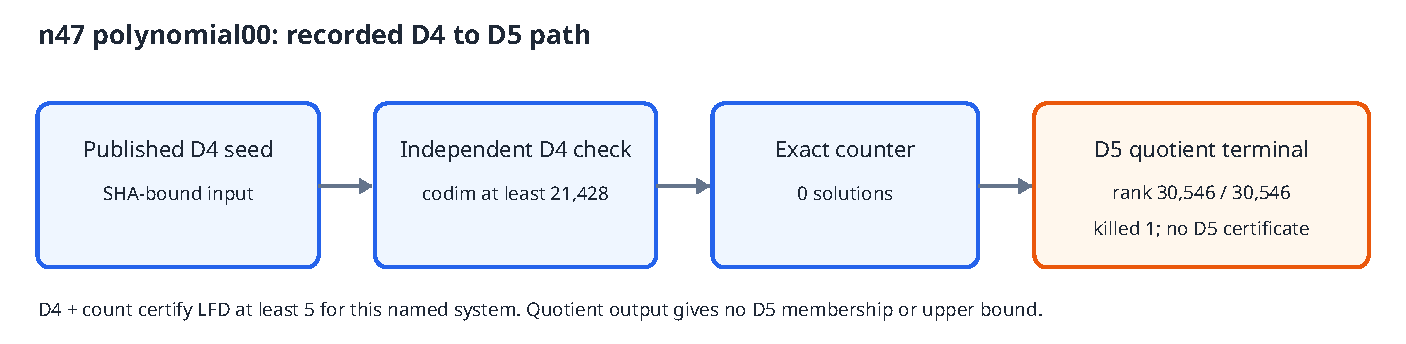
\includegraphics[width=\linewidth]{flow.pdf}
\end{center}
\small{The diagram separates independently checked D4/count evidence from the native D5 quotient observation.}

\paragraph{Custody and scope.} \texttt{readback.json} records full GET hashes for 14 small S3 objects and checks the D4 transcript, exact count, native terminal status, and absence of checkpoint manifests. The pod exited 0 with zero restarts. Stage wall times were marked invalid for comparison. A degree-six lower bound requires an independently accepted D5 certificate with checked codimension above the exact solution count.
\end{document}
